\chapter{Introduction}

Almost everyone uses the internet daily, whether connecting to it from their mobile devices or browsing it on their personal computers. Therefore, it is safe to say that most of us will struggle with everyday activities without internet communication devices. For example, getting a taxi ride, ordering food deliveries or even navigating to places we want to go. Apple made an interesting short movie, "predicting" what might happen without Apps on mobile devices during their annual Worldwide Developers Conference \textbf{(WWDC)} in 2017 \cite{int1}.
 
The internet has an even greater presents and role within the science and engineering community. For example, sites like Google Scholar and The New England Journal of Medicine have greatly benefited scientists, doctors, and engineers \cite{int2} \cite{int3}. Before the wide adaption of the internet, researchers, scholars and students would spend countless hours in physical libraries, browsing through hundreds of academic journals and books to answer one question or solidify a proposal they had in mind. Today, with the help of the internet, it will hardly take a few minutes. This leads to a jump in research productivity, which helps researchers and engineers produce their research and production output to a new level, thus allowing them to do more things in the same amount of time.

\bigskip
\section{Introduction to JavaScript and the history of the web}

For the last 20 years, JavaScript has been the technology that dominated the majority of web browsers and the web development industry. Although updates and new versions are issued regularly, they are still becoming more aged daily. Software engineers have been finding ways to improve this ageing technology's runtime performance, user experience, and developer experience. For example, Microsoft developed the Typescript language to combat the "strange" nature of JavaScript and to help resolve the lack of type checking within JavaScript \cite{int4} \cite{int5}. Facebook developed the "React" library framework to improve the developer experience by introducing the "component" concept. Where each class or function within a React project can be seen as a UI (user interface) component, this can be a button, a table or a component with more complexity, such as a navigation header component \cite{int6}. As expected and intended, some of the popular web development frameworks and libraries, such as \textbf{React JS} and \textbf{Angular}, developed by Google have gained significant attention and much of the industry-wide adaption since their release, and they have indeed significantly improved the browsing experience for all of us.

There is a widespread misconception that Al Gore, the Former Vice President of the United States, invented the internet. However, this is false, as Al Gore has never claimed or said so. Instead, what he actually said was, "I took the \textbf{initiative} in creating the internet" during his interview with CNN in 1999 \cite{int7}. However, Al Gore did introduce the High Performance Computing Act of 1991 \cite{int8}, which helped fund the creation of the first mainstream web browser Mosaic \cite{int9}, as well as the creation of the high-speed fibre optic computer network \cite{int10}.

JavaScript was born not long after the release of the first version of Netscape Navigator - the most popular web browser in the late 90s. It was written by Brendan Eich, and it only took him 10 days to release the very first version \cite{int11}. Initially, JavaScript did not gain that much attention, and it wasn't until the release of Internet Explorer version 3 which added support for the language. After that, the popularity of JavaScript increased dramatically among the general public \cite{int12} \cite{int13}. Growing up alongside the internet, JavaScript has undergone several iterations and feature upgrades. Although it is indeed powerful and popular, however, in recent years, developers and engineers started to see JavaScript as a "messy" language [figure \ref{fig:javascript_meme}]. During this period, another popular web technology - Adobe flash player- was gradually replaced by its newer counterpart - HTML 5. This is primarily due to its performance and security issues \cite{int14}. Between 2011 and 2021, the percentage of websites using Flash dropped from 28.5 per cent to just 2.2 per cent \cite{int15}. Adobe, alongside other popular web browsers, formally ended the support and update for Flash in 2021 \cite{int16}.

A significant change was just around the corner.

Developers and major tech companies started forming the future of the web. They wanted a new technology standard that aligned with the current web application development trend and laid the groundwork for the industry's future. After much discussion, they devised the idea of creating a brand new language based on all the experiences and mistakes from the last 20 years. Thus, in 2017, we were introduced to the WebAssembly language.

\newpage
\bigskip
\begin{figure}[hp]
\centering
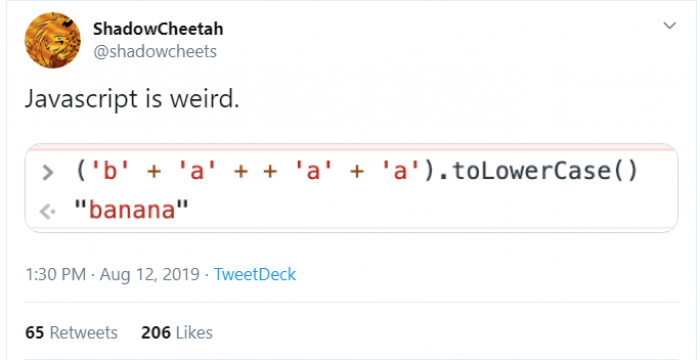
\includegraphics[scale=0.7]{javascript_meme}
\caption{\footnotesize{Internet "meme" about the JavaScript language. \cite{inta1}}}
\captionsetup{aboveskip=0pt,font=it}
\label{fig:javascript_meme}
\end{figure}
\bigskip

\bigskip
\section{Meet WebAssembly}

After its initial release in 2017, WebAssembly was first adopted by a number of major web browsers \cite{int17}. Since then, there has been a growing community built around the technology as more and more projects have started using WebAssembly. As mentioned above, JavaScript has been the de facto language for web browsers since the beginning of the web. However, this was never the original intention during the development of JavaScript.

WebAssembly is the first widely adopted language built entirely from the ground up with formal semantics, and it was designed to work in areas it originally intended, which are large, complex interactive applications running on modern web browsers. It has an immaculate, simple yet powerful design such as memory allocation and garbage collection \cite{int18}. However, WebAssembly is actually a form of binary code. Developers and engineers don't usually write WASM code directly; instead, they write programs with other low-level languages such as c, c++ or rust, which will then be compiled down to WebAssembly code \cite{int19}.

One of the most significant advantages of WebAssembly is standardisation. That is the ability to compile a wide variety of different programming languages down to just one, which can be very useful in many different scenarios. The industry term of this practice is called \textbf{polyglot}, and it is largely missing from today's software development practices \cite{int20}. As an example, Java and Python developers cannot work on the same piece of software together because the code compilation method is different between the two languages. However, when it comes to developing WebAssembly programs, developers from all programming backgrounds have the ability to work together and contribute to the same piece of software using languages they are comfortable with. One good example of this method is Microsoft's ASP.NET framework \cite{int21}. ASP.NET, sometimes also referred to as the .NET framework family, was one of the first consumer-facing web frameworks for building web applications. It was released in 2002 alongside the Visual Basic programming language \cite{int22} \cite{int23}.

The VB language was popular for a time in the early 2000s, however, after a few years of its initial release, engineers at Microsoft decided to switch their primary language for .NET development from VB to C\#. This is primarily due to C\# being an elegant language with modern syntax \cite{int24}. However, instead of suddenly ending the support for Visual Basic language, they developed new versions of the .NET runtime to support and run a mixture of both languages \cite{int25}. This way, not only developers who work in different languages can operate together. But more importantly, big, legacy applications can be continuously developed to extend their service life.

\bigskip
\begin{figure}[hp]
\centering
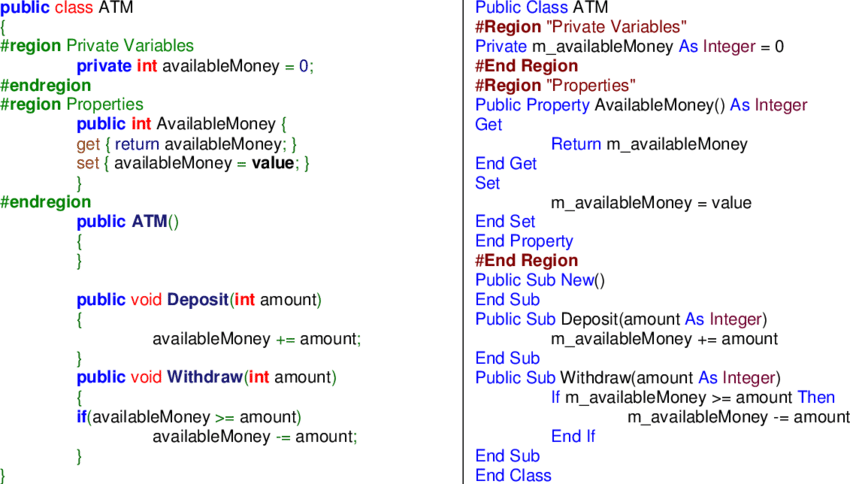
\includegraphics[scale=0.5]{C-to-VBNET-code-conversion-C-source-code-VBNET-source-code}
\caption{\footnotesize{Syntax between C\# (left) and VB (right) \cite{int26}}}
\captionsetup{aboveskip=0pt,font=it}
\end{figure}
\bigskip

\newpage
\section{Use cases of WebAssembly}

As we mentioned above, since 2017, the four most prominent web browsers have all been developed to compile and render WebAssembly out-of-the-box. And since then, the popularity of WebAssembly within frontend web development has increased dramatically. However, in this thesis, we will be looking into and conducting research and study on one of the latest use cases of WebAssembly - server-side WebAssembly development.

The modern, well-loved features of WebAssembly, combined with the release of the WebAssembly system interface, made it all possible to move WebAssembly outside of web browsers to be run on other environments. Soon, scientists and engineers formed the idea of building a WebAssembly runtime that allows it to run natively on popular operating systems such as Windows, Mac OS and Linux, just like what Node.js runtime allowed JavaScript to achieve \cite{int27}.

This is a considerable achievement for WebAssembly because by being able to write applications that can run natively on operating systems, we can unleash the true power of WebAssembly. Take Node.js, for example, before it was released, the developer experience for desktop applications needed to be better, and there were very few options to develop cross-platform desktop applications. Soon after its release to the public, companies started to create new applications with Node.js frameworks or migrate their existing applications and services to Node.js. As a result, some of the most popular desktop applications used by many of us daily are now written in Node.js, such as Slack, Zoom and WhatsApp \cite{int28} \cite{int29} \cite{int30}.

For any new technology that wants to be successful and gain popularity among developers and engineers, it needs to outperform its competitors in some ways to convince the industry that it can be faster, more powerful, more reliable or more accessible to develop than the technology it intends to replace. Node.js provides a familiar development environment to web developers since it was built on top of Google's V8 browser rendering engine \cite{int31}. On top of that, it has an easier learning curve, and it also performs better than most desktop application frameworks at the time, such as Windows Presentation Foundation (WPF), Universal Windows Platform (UWP) and Java Swing \cite{int32} \cite{int33} \cite{int34}.

\newpage
\bigskip
\begin{figure}[hp]
\centering
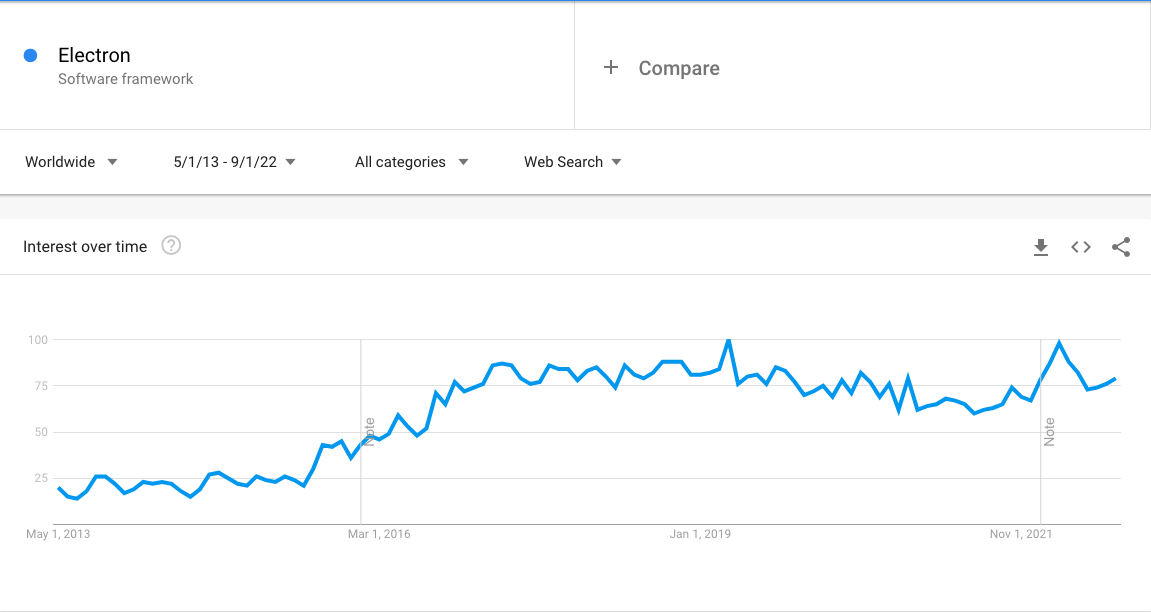
\includegraphics[scale=0.3]{electron-trend}
\caption{\footnotesize{Increase in popularity of the Electron framework since released in 2013 \cite{exp1}}}
\captionsetup{aboveskip=0pt,font=it}
\end{figure}
\bigskip

Similarly, WebAssembly running on a native OS is intended to improve the existing Node.js solution to deliver an even better experience for both users and developers. One of the biggest challenges for Node.js applications is the amount of memory it uses \cite{int35}. Although fast and agile, Node.js applications and the Google Chrome browser have been long criticised for their intense memory usage \cite{int36}. A recent study showed that Google Chrome uses 10 times more memory than Apple's Safari browser when running natively on macOS Big Sur operating system \cite{int37} \cite{int38}.

\newpage

\bigskip
\begin{figure}[hp]
\centering
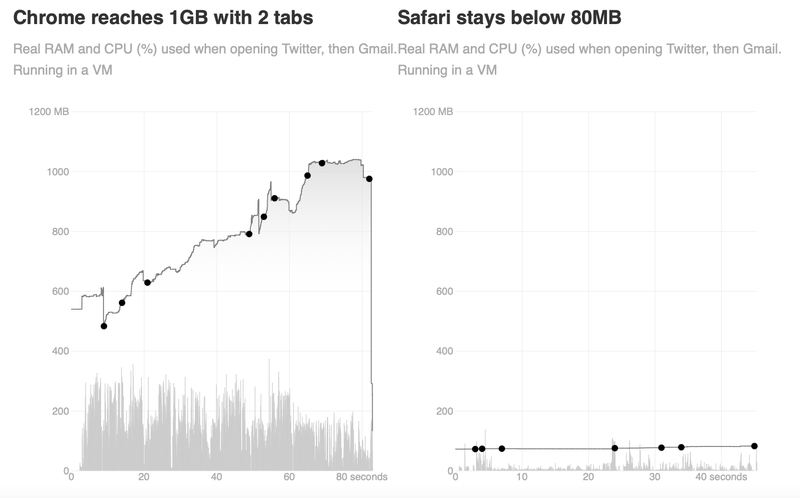
\includegraphics[scale=0.4]{chrome-safari-ram-test}
\caption{\footnotesize{Safari vs. Chrome on memory and CPU usage comparison 1 (VM) \cite{int39}}}
\captionsetup{aboveskip=0pt,font=it}
\end{figure}
\bigskip

\bigskip
\begin{figure}[hp]
\centering
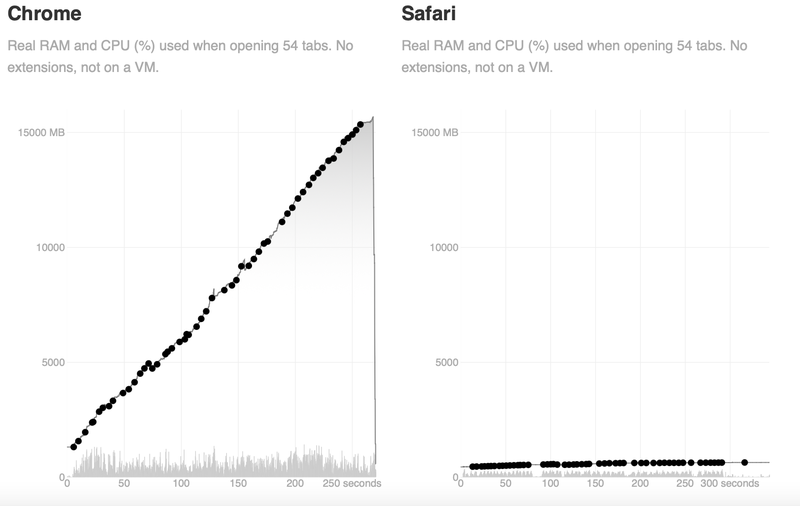
\includegraphics[scale=0.4]{chrome-safari-RAM-2}
\caption{\footnotesize{Safari vs. Chrome on memory and CPU usage comparison 2 (Native) \cite{int39}}}
\captionsetup{aboveskip=0pt,font=it}
\end{figure}
\bigskip

As we see in the above figures, with only two browser tabs open, Google Chrome already used 1 GB of memory, and when running 54 browser tabs, Google Chrome uses 24 times more memory than Safari.

Issues like this are precisely what WebAssembly intends to tackle and resolve. For example, benchmark testing showed that when comparing the download size and memory usage between Electron Node.js and Microsoft's Blazor WebAssembly desktop applications, Node.js can be up to 82.5 times larger in terms of download size and uses 7.9 times more memory than its WebAssembly counterpart \cite{int40}.

\bigskip
\begin{figure}[hp]
\centering
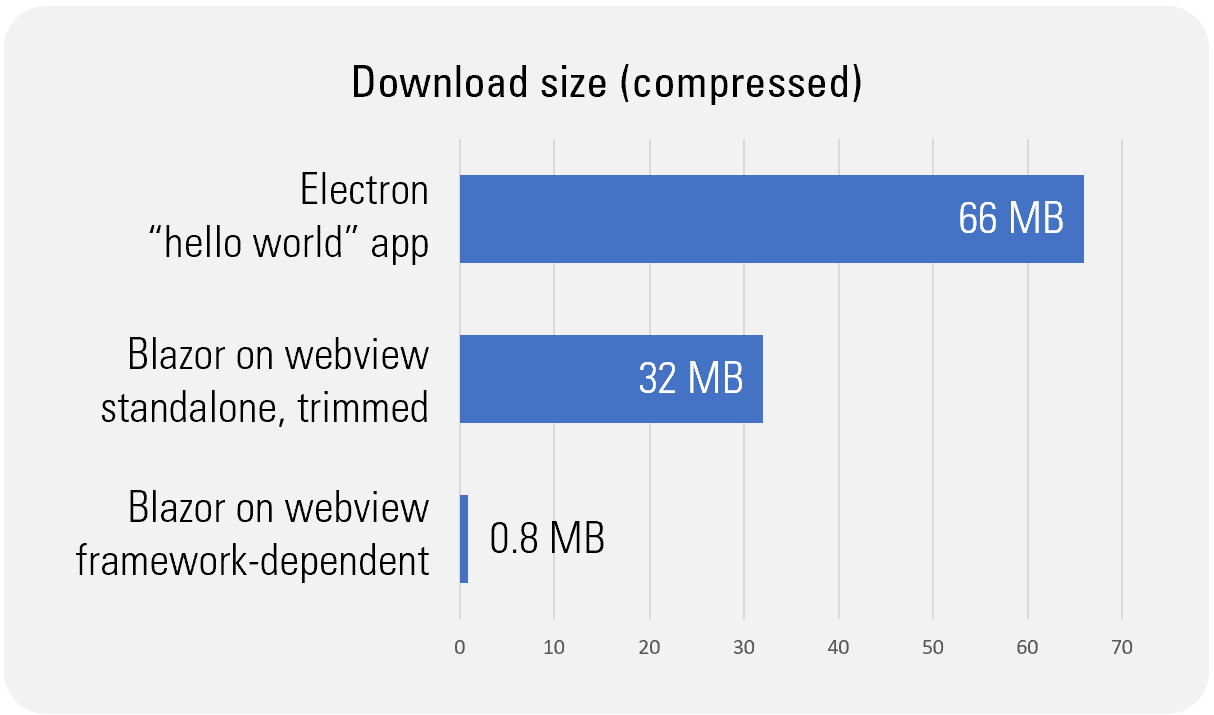
\includegraphics[scale=0.9]{download-size-chart}
\caption{\footnotesize{Electron vs. Blazor on package size comparison \cite{int40}}}
\captionsetup{aboveskip=0pt,font=it}
\end{figure}
\bigskip

\bigskip
\begin{figure}[hp]
\centering
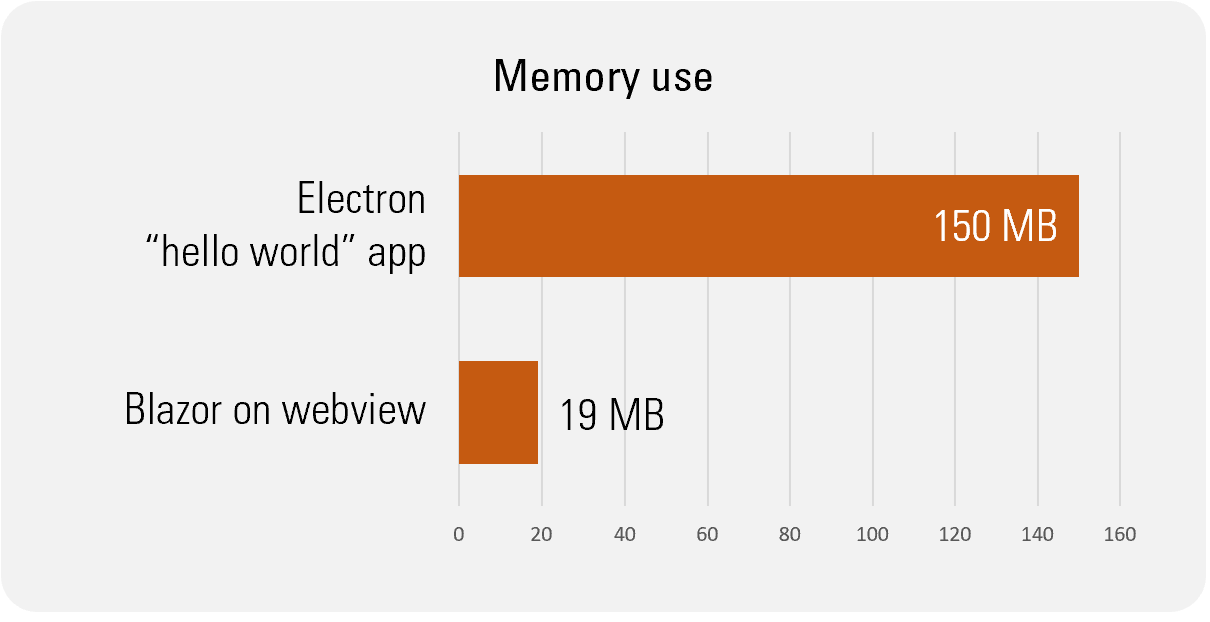
\includegraphics[scale=0.9]{memory-use-chart}
\caption{\footnotesize{Electron vs. Blazor on memory usage comparison \cite{int40}}}
\captionsetup{aboveskip=0pt,font=it}
\end{figure}
\bigskip

\section{Outline of the Thesis}
\bigskip

In this thesis, we will conduct studies and investigations on the performance gap and inconsistency between applications running with VM/Containers in the cloud and applications built with WebAssembly frameworks running on the edge. First, we will uncover the pros and cons of this new way of developing cutting-edge, low-latency applications. After that, we will undertake our experiment with the two frameworks of our choice. And finally, deliver our verdict on the current state of WebAssembly running on the edge for commercial use.

In \textbf{\autoref{chap:litreview}}, we will provide a detailed literature review on related background work, including research and studies that have already been done within this area, as well as the proposed further studies. Then in \textbf{\autoref{chap:methodology} and \autoref{chap:background}}, we will formally introduce our experiment, including the overview, the background, the procedure and the expected outcome. After that, in \textbf{\autoref{chap:experiments}}, we will formally conduct the experiment to compare and study the difference in performance and behaviour of the two frameworks of our choice. Next, we will present the result and findings in \textbf{\autoref{chap:results}}. After that, we will provide our verdict on the experiment outcome through a discussion in \textbf{\autoref{chap:discussion}}. Finally, we will summarise the experiment and our findings within it, provide suggestions on further research, and deliver final remarks.